\noindent L-pad resistive networks are typically used for very broadband impedance matching in applications where a significant amount of insertion loss can be accepted (e.g. 50 $\Omega$ to 75 $\Omega$ matching pads).

  \begin{figure}[ht]
    \centering
    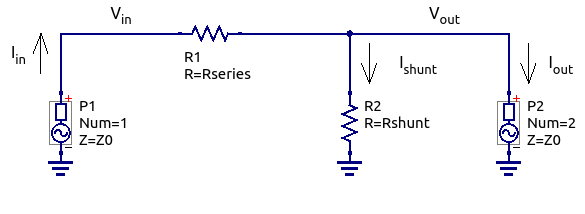
\includegraphics[width=10cm]{./images/l-pad-series-attenuator-schematic.png}
    \caption{L-pad series attenuator}
    \label{fig:l-pad-series-attenuator-schematic}
  \end{figure}
  
\noindent As before, the design equations can be obtained through network analysis. Being $I_{in} = I_{shunt} + I_{out}$. Provided that:

  \begin{equation}
  	\begin{cases} I_{shunt} = \frac{Vout}{R_{shunt}} \\ I_{in} = - \frac{V_{in}}{Z_0} \\ I_{out} = \frac{V_{out}}{Z_0} \end{cases}
  \end{equation}
  
\noindent Combining these equations into the first one, we get that the voltage gain is:

\begin{equation}
	A_v = \frac{V_{out}}{V_{in}} = -\frac{R_{shunt}}{Z_0 + R_{shunt}}
\end{equation}

\noindent Provided that the attenuation (in natural units) is related to the voltage gain as $\alpha^{n.u.} = A_v^2$, the following expression holds:

\begin{equation}
	(1 - \alpha^{n.u.}) \cdot R_{shunt}^2 - 2 \cdot \alpha^{n.u.} \cdot Z_0 \cdot R_{shunt} - \alpha \cdot Z_0 = 0
	\label{eq:L-pad-series-equation}
\end{equation}

\noindent Eq. \ref{eq:L-pad-series-equation} has two solutions:

\begin{equation}
	\begin{cases}
		R_{shunt}^{S1} = \frac{- Z_0 \cdot (\alpha^{n.u.} + \sqrt{\alpha^{n.u.}})}{\alpha^{n.u.} - 1} & \text{Solution 1} \\
		R_{shunt}^{S2} = \frac{- Z_0 \cdot (\alpha^{n.u.} - \sqrt{\alpha^{n.u.}})}{\alpha^{n.u.} - 1} & \text{Solution 2}
	\end{cases}
\end{equation}

\noindent A valid solution must also satisfy the input match condition:

\begin{equation}
	Z_0 = R_{series} + R_{shunt} \parallel Z_{load} \Rightarrow R_{series} = \frac{Z_0^2}{Z_0 + R_{shunt}}
\end{equation}

\noindent Each solution for $R_{shunt}$ is related to a $R_{series}$ value:

\begin{equation}
	\begin{cases}
		R_{series}^{S1} = -Z_0 \cdot \frac{\alpha^{n.u.} - 1}{\sqrt{\alpha^{n.u.}} + 1}  & \text{Solution 1} \\
		R_{series}^{S2} = Z_0 \cdot \frac{\alpha^{n.u.} - 1}{\sqrt{\alpha^{n.u.}} - 1} & \text{Solution 2}
	\end{cases}
\end{equation}

\noindent Provided that $\alpha^{n.u.} < 1$, Solution 1 is always valid since $R_{shunt}, R_{series} > 0$. Solution 2 yields negative resistor values.

\noindent The output impedance of the L-pad can be obtained as follows:

\begin{equation}
	Z_{out} = R_{shunt} \parallel \left( R_{series} + Z_0 \right) = \frac{R_{shunt} \cdot \left( R_{series} + Z_0 \right)}{R_{shunt} + R_{series} + Z_0}
\end{equation}

\noindent Concerning power dissipation in the resistors, the following expressions were obtained:

\begin{equation}
	P_{diss}^{R_{series}} = P_{in} \cdot \left( 1 - \sqrt{\alpha^{n.u.}} \right)
\end{equation}

\begin{equation}
	P_{diss}^{R_{shunt}} = P_{in} \cdot \alpha^{n.u.} \frac{1 - \alpha^{n.u.}}{\alpha^{n.u.} + \sqrt{\alpha^{n.u.}}}
\end{equation}